\chapter{Introduction}

%The story  I want to tell explains the Casimir force via its historical origins which serve to introduce the big results, while sidestepping weird irrelevant bullshit.  I want to hit the important context for modern scientists and emphasize quantities realted to current experiments.  I also want to outline the currently available most powerful methods to set context for what else is possible, and what its limitations are.  

%I think I can do this with a partial historical introduction.

\begin{itemize}
\item General thesis about quantum physics of atoms using computation.  
\item Thesis covers numerical monte-carlo techniques, where random numbers used in simulation.
\item First new method for computing electromagnetic Casimir energies.
\item Second, continuous position measurements of atoms taking into account experimental constraints.  
\item United in perspective of numerical work relying on Monte-Carlo techniques, to explore quantum phenomena relevant to modern experiments and pushes toward future technology  
\end{itemize}



\section{Casimir Forces in general and physical interpretation}

\begin{itemize}
\item Casimir force arises due to fluctuations in quantum fields. 
\item Forces between macroscopic bodies, atoms and bodies and between atoms.  
\item Interesting for theory reasons as purely quantum field theory phenomena, and relevance to current experimental physics.  
\end{itemize}


\begin{itemize}
\item General references Cite Books - Milonni~\cite{Milonnibook1994}, Milton~\cite{Miltonbook2001}.  Bordag~\cite{Bordagbook2009}, Dalvit~\cite{Dalvitbook2011} recent developments.  
\item More general books on Casimir and van der Waals forces as they relate to chemistry , Parsegian~\cite{Parsegian2006}, Israelachivili~\cite{Israelachvili2011}.
\end{itemize}


\subsection{Casimir energy}

The Casimir force is an attractive force that arises due to fluctuations in quantum fields.  It was first predicted in 1948 by Henrik Casimir~\cite{Casimir1948}.  If we consider two planar perfect conductors, we find that there is an attractive force between them due to the zero point energy of the electromagnetic field.  In a quantum electrodynamics the ground state of each mode of the electromagnetic field contributes $\hbar\omega/2$, where $\hbar$ is Planck's constant, and $\omega$ is the frequency of the mode.  The presence of the conductors forces the electric field to vanish on the surfaces, which restricts the allowed modes of the electromagnetic field. If we add up the energy from all modes of the electromagnetic field, and compare it to the case when the plates are infinitely far apart from one another, we find the energy is reduced as the plates are brought closer together.  The energy between the plates is then
\begin{equation}
  E = -\frac{\hbar c}{240\pi^2 d^3},
\end{equation}
where $c$ is the speed of light in vacuum, and $d$ is the distance between the plates.

\subsubsection{Calculation for perfect conductors}

\comment{Give simple derivation of force? Cite Bordag/Dalvit?}
Reprise original Casimir calculation~\cite{Casimir1948}.  
\begin{itemize}
\item Mode functions
\item Energy integrals, changes of variable
\item Renormalization
\end{itemize}

\begin{figure}
\center
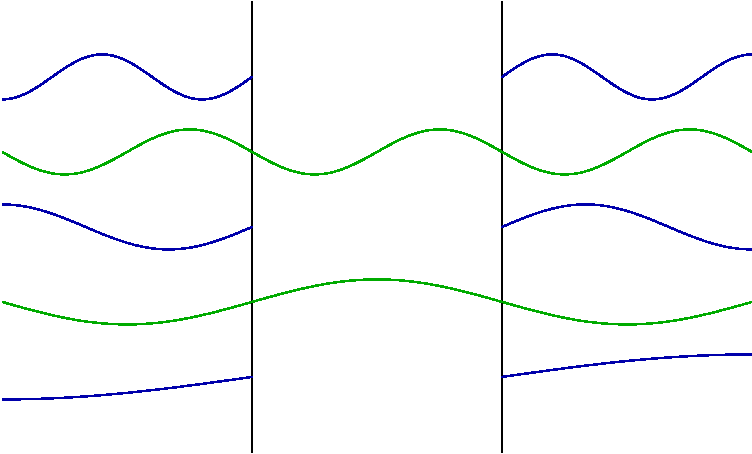
\includegraphics[width=10cm]{fig/intro/twoplanes_wave}
\caption{Sketch of allowed modes between perfectly conducting plates.}
\end{figure}


\subsection{Casimir-Polder energy}

The Casimir force is also important for atoms near surfaces.  This variant is known as the Casimir-Polder force, after a paper by Casimir and Polder where they computed the force between an atom and a perfect conductor accounting for the finite speed of light~\cite{CasimirPolder1948}.  
In this case, the atom feels an attractive potential to a surface a distance $d$ away,
\begin{equation}
V_{CP} =-\frac{3\hbar c\alpha_0}{64\pi^2\epsilon_0 d^4}.
\end{equation}

\comment{Note Dan's notes as example calculations.  }

\subsection{Van der Waals forces}

The formalism was extended to include dielectric media by Lifshitz~\cite{Lifshitz1956}.  \comment{He also worked alongside co-workers Dzayolshinkii and Abrisokov to further compute the force from using Feynman diagrammatic methods\cite{Dzyaloshinskii1959,Dzyaloshinskii1961}}.  
\comment{Point of view: Due to thermal fluctuations in medium.}

\comment{Mclachlan\cite{Mclachlan1963} cites these guys?}

\comment{Barton?}

\subsection{Scale and Physical Interpretation}

\begin{itemize}
\item Ground state energy or zero point enery.  Emphasizes boundary conditions and restricted spectrum of fluctuations.  
\item Atoms emitting and absorbing virtual photons.  
\item Feynman Diagram.  
Atom-Wall
\begin{figure}
  \centering
\begin{fmffile}{atom-loop}
  \begin{fmfgraph*}(100,60)
    \fmfleft{i}
    \fmfright{o}
    \fmftop{t}
    \fmf{plain}{i,v1}
    \fmf{plain}{v2,o}
    \fmf{plain,label=$|e\rangle$}{v1,v2}
    \fmf{photon,left=0.5,tension=.4}{v1,vt,v2}
    \fmf{phantom,tension=1}{t,vt}
    \fmflabel{$|g\rangle$}{i}
    \fmflabel{$|g\rangle$}{o}
    \fmflabel{$\gamma$}{vt}
  \end{fmfgraph*}
\end{fmffile}
\caption{Atom interacting with wall via emitting and absorbing photons.  }
\end{figure}

Wall-Wall Effective action.

\begin{figure}
\centering
\begin{fmffile}{wall-wall}
\begin{fmfgraph}(50,30)
 \fmftop{t0,t1,t2,t3}
 \fmfbottom{b0,b1,b2,b3}
 \fmf{phantom}{t1,v1}
 \fmf{phantom}{t2,v3}
 \fmf{phantom}{b1,v2}
 \fmf{phantom}{b2,v4}
 \fmffreeze
\fmf{photon}{v1,v3}
\fmf{photon}{v2,v4}
\fmf{fermion,tension=0}{v1,v2}
\fmf{fermion,tension=0,left}{v2,v1}
\fmf{fermion,tension=0}{v3,v4}
\fmf{fermion,tension=0,right}{v4,v3}
\end{fmfgraph}
\end{fmffile}
\caption{Casimir Energy in terms of fundamental QED processes.  Electrons are considered bound within their respective media.}
\end{figure}

\item Picture of Electrons interacting with EM field.  Effective action at some loop order in basic QED.  Makes contact with fundamental physics.  Can then make sense of limits in which we are operating.  Doing perturbation theory on QED.  $\epsilon$ is linear response of medium to EM field, and working to leading order in $\epsilon$.  Amounts to $\order(\alpha_0^4)$ diagram for QED with electrons bound via nuclear potential.   (Again, very low energies).
\begin{itemize}
\item Assuming electrically neutral
\item Far from atomic separations, so continuum approximation acceptable.
\end{itemize}

\item Casimir forces are short ranged forces and decay away quickly.  The Coulomb potential between charged particles is behaves as $d^{-1}$, where $d$ is the particles separation.  In comparison, the London dispersive force between two atoms decays as $d^{-7}$.  For macroscopic bodies, the decay is slower, since we can roughly think of adding up the contributions from all of the constituent atoms.  For Casimir energies, the energy decays as $d^{-3}$.  

These considerations are for zero temperature.  It turns out that considering the effects of finite temperature, in particular thermal photons, leads to different distance dependence again.  The energies typically decay more slowly in the high temperature limit.  If the Casimir force decays as $d^{-n}$ at zero temperature, then we typically find that the force decays as $r^{-n+1}$ at high temperatures.  

We can estimate typical distance scales by considering the dominant resonances of the medium, and the thermal wavelength.  So the Casimir force is typically then important at distances below the transition wavelength which is usually around $1\mu m$.    

\item The typical energy scale can also be estimated.  If we consider an atom with a static polarizability of $\comment{polarizability}$, at a distance of $1\mu m$, we find the Casimir-Polder potential is \ldots. 

For macroscopic bodies we can compare the Casimir energy for perfect metal conductors at a distance $d$ to the energy stored in the capacitance.  Note that we compute an energy per unit area.  

The Casimir energy per unit area is $\frac{\hbar c\pi^2}{240 d^3}$, while the voltage for a parallel plate capacitor is.
\begin{shaded}
\begin{itemize}
\item Capacitance is $V=Q/C$.  
\item $C = \epsilon_0 A/d$.  
\item Energy is $\frac{1}{2}CV^2=\frac{Q^2}{2C} $
\end{itemize}
\end{shaded}

\end{itemize}


\begin{itemize}
%\item Cite Casimir/Casimir-Polder and Lifshitz.
\item Casimir vs Van Der Waals vs London Forces

The Casimir force is intimately related to the van der Waals forces between molecules.  Van der Waals forces are usually ascribed to the dipole fluctuations of the neutral atoms.  In the limit where the atoms are far apart retardation becomes important and the force changes decays more quickly as $r^{-7}$.  In this limit the forces are sometimes referred to as London dispersion forces.  Normally Casimir forces consider the 

Throughout this thesis we shall use Casimir forces to refer to the forces between macroscopic bodies, and Casimir-Polder forces to refer to the forces between atoms and macroscopic bodies.  

\item Renormalization

As QED calculation, the Casimir energy is formally divergent and must be renormalized.  In our case, we typically energy differences when one of the bodies is removed to spatial infinity.  In some cases, like spheres we must consider renormalization more carefully.  In those cases, the formally infinite parameters we get renormalize the physical parameters of the model~\cite{Miltonbook2001}.  

\item Non-additivity of forces:  Reference for this?  What is the typical scale of the correction for non-additivity?

\item Search for repulsive forces

\begin{itemize}
\item Casimir force important for stiction.
\item Attracts atoms, sets lower bound for how close you can get particles together.
\item Search for repulsive forces as possible trapping (Motivation for this?)
\item Can be found for magnetic media (but typically small).  Metamaterials exhibit this for small range of frequencies.  But Casimir broadband, and dielectric contribution ends up dominating.  (\comment{ Cite Milonni on metametarials}.Sufficiently anistropic dielectric media (how anisotropic? \comment{Cite Milton}) $\epsilon_1<\epsilon_3<\epsilon_2$ over a broad enough range of frequencies \comment{Cite Lifshitz of liquid helium.  Cite experiments, and note odd fluids.}.   Geometries dependence (\comment{Cite reid paper on needle above hole}).
\end{itemize}
\item Dynamical Casimir effect/Unruh Effect?
\begin{itemize}
  \item Accelerating plate creates photons.  L
\end{itemize}
\end{itemize}

\section{Physical relevance and experimental relevance}

\section{Experiments}
\subsection{Physics}
\begin{itemize}
\item Liquid Helium
\item Spaarnay
\item Lamoreaux - for 1997 measurements\cite{Lamoreaux1997}, and also recent thermal work by Sushkov\cite{Sushkov2011}.

\item Mohideen \cite{Mohideen1998} AFM with sphere above plate.

\item Capasso \cite{Chan2001}  torsion oscillator above plate
\item Bressi \cite{Bressi2002} Parallel Plates.
\item Cornell - atoms near wall\cite{Harber2005, Obrecht2007}.  BEC near wall, detect change in oscillation frequency of trap due to Casimir-Polder energy.  Using thermal shift?
\item Antezza - chapters in Dalvit.  
\item Kimble atoms near toroidal resonators.  \cite{Alton2011}.  Atoms above 1D Microcavity \cite{Hung2013}
\item Atom-chips  Schmiedmeyer\cite{Folman2000,Schneider2003}(?)  Not explicitly using Casimir-Polder forces?  
\item Cronin \cite{Perreault2005,Lonij2009}  Atom interferometry experiments for atoms near gratings.
\item Sukenik\cite{Sukenik1993}, atoms passing through cavity to detect Casimir-Polder.  
\end{itemize}

\begin{itemize}
\item Controversies about role of zero temperature pole.  
\item Lamoreaux favors Drude model, Capasso favours plasma model.
\item Seems experiments favour more 
\end{itemize}

\subsection{Chemistry/Helium/Geckos?}

\begin{itemize}
\item Geckos use the Casimir force \cite{Autumn2002}.
\end{itemize}

\subsection{Modifications to gravity}

\begin{itemize}
\item Modifications to gravity on $1\mu m$ or $1mm$ scale.  Cite Lamoreaux 2000 Paper.  Gervaci?
Yukawa type forces.  
\item Subtract off Casimir force background.  Tino group.  Use Casimir shield with fairly thick gold to have same Casimir force, and thne vary the medium behind it.  Longer range gravity should lead to 
Requires very careful measurements, on top of carefully extracting Casimir force.   
\end{itemize}

\section{Other Computational methods}

\subsection{Proximity Force Approximation}

\begin{itemize}
\item Find first use?  Lamoreaux mentions usage.  Derjaguin?
\item Note problem with non-additivity. 
\item Good as order of magnitude estimate?  Useful if very limited curvature, or effectively approximate geometry as planar.  
\end{itemize}

\subsection{Green function methods}

\begin{itemize}
\item Cite Schwinger~\cite{Schwinger1978, Milton1978}  Scalar green functions.  
\item Green tensor methods
\item Cite Barton
\item Cite Philbin(?)
\item Cite Vogel and Welsch
\end{itemize}

\subsection{Reflection Matrix}

\begin{itemize}
\item Cite Balian and Duplantier \cite{Balian1977, Balian1978}.
\item Cite Lambrecht and French collaborators
  \cite{Lambrecht2006, MaiaNeto2008,Canaguier-Durand2012}
\item Cite Milton
\end{itemize}

\subsection{Scattering Matrix Path Integral Methods}

\begin{itemize}
\item Physical Picture based on generalized Green theorem from SIE~\comment{Stratton}.
\begin{itemize}
\item What are the SIE ?  
\item Comment on Emig/Buscher showing you can use homogenous green function.  Relation to Green's theorem.
\end{itemize}

\item Cite Emig,Jaffe,  and others for initial analytical techniques.  Relies on Green theorem.
\cite{Emig2004, Emig2007, Rahi2009}
\item Cite Johnson/Reid/ for numerical progress.  Note use of existent analytical methods and similarities to existent numerical FTDT techniques on earlier papers.  \cite{Reid2009,Reid2011, Reid2013} \cite{Rodriguez2007,Rodriguez2007a, Rodriguez2009}
\item Note success, applicability.  \comment{Cite experimental tylenol pill paper}
\item Estimates on scaling of algorithm?
\end{itemize}

\subsection{Worldlines}

The worldline method is an alternative method for computing Casimir energies.  The worldline method was initially developed as an alternative method for carrying out QFT calculations in terms of particle mechanics~\cite{McKeon1993, Strassler1992,Schubert2001}.  In particular we can compute compute quantum effective actions in terms of the suitable dynamics of a quantum particle.  \comment{Other references - was one contemporaneous with Strassler? Bern-Kosower}

The basic insight is that for one loop effective actions, we can recast a field path integral calculation in terms of the particle path integral for particles travelling in closed space-time loops.  This is quite similar to the scalar electrodynamics Feynman explored in his Ph.D thesis~\cite{Feynman1942, Brown2005}\comment{Seems to actually be his 1950 QED paper RE Schubert2001}.  Higher order loop calculations can also be carried out with more particles, and gauge fields can also be treated~\cite{Schubert2001}.  For example, the worldline method has been used to compute relativistic field effects for QED such as the Lamb shift~\cite{Schmidt1995}.  It has also been used as a numerical algorithm\cite{Mazur2014}.

The worldline method is heavily based on Feynman's path integral method~\cite{Feynman1948,Feynman1965}.

Our primary interest in the worldline method is for computing Casimir energies, which can be cast as effective actions.  The worldline was first used for the Casimir energy by Gies\etal~\cite{Gies2003,Gies2006, Gies2006a}.  While the initial work focused on the zero temperature limit, the worldline method has also been extended to finite temperatures~\cite{Klingmueller2008}.  This has also been used to study the torsion of inclined planes~\cite{Weber2009}, and planes and spheres and planes and cylinders~\cite{Weber2010, Weber2010a}.  

We will briefly introduce the method here, and discuss the method at length in Ch.~\ref{ch:scalar_worldlines}.  Let the action for the scalar field be given by 
\begin{equation}
  S = \int_0^T dt \int d^3x \left[ (\partial_t\phi)^2-(\nabla\phi)^2-V(\vect{x},t)\phi^2\right],
\end{equation}
where $V(\vect{x},t)$ defines the surfaces of the objects we wish to compute the Casimir energy between.  The potential is typically chosen to be $V(\vect{x},t)=\lambda\delta[\sigma(\vect{x})]$, where $\sigma(\vect{x})=0$ defines the surfaces.  In the limit $\lambda\rightarrow\infty$ the potential enforces Dirichlet boundary conditions, where $\phi(\vect{x})\big|_{\sigma(\vect{x})=0} =0$.  This corresponds to assuming the surfaces are idealized perfect conductors.  

We can compute the partition function for the field by Wick rotating to imaginary time (or finite temperature), where the partition function is now given by 
\begin{equation}
  Z = \int D\phi \exp\left\{-\int_0^T dt \int d^3x \left[ (\partial_t\phi)^2+(\nabla\phi)^2+V(\vect{x},t)\phi^2\right]\right\},
\end{equation}
The Gaussian integration over fields can be carried out as a functional determinant.  In order to compute the energy we need the logarithm of the partition function, and various derivatives of it.  The end result of these manipulations is that the renormalized energy can be written as 
\begin{equation}
E_{\text{scalar}} = \frac{\hbar c}{(2\pi)^{D/2}}\int_0^\infty \frac{d\cT}{\cT^{1+D/2}} \int d\vect{x} \dlangle e^{-\cT\langle V\rangle} -1\drangle,
\end{equation}
where $\cT$ is the loop ``time'' and governs the extent of the loops, $\vect{x}_0$ is the loop starting point, $\dlangle \cdots\drangle$ denotes an ensemble average over closed Gaussian random walks, and $\langle\cdots\rangle$ denotes the average of a quantity around the loop.  


\begin{figure}
\center
\includegraphics[width=10cm]{fig/intro/hit_strong_coupling}
\caption{Upper loop touches both objects and will contribute to Casimir energy.  Lower loop only touches one body, and does not contribute to Casimir energy.}
\end{figure}



\begin{itemize}
%\item Cite Schubert~\cite{Schubert2001}, Strassler~\cite{Strassler1992} on general worldline
% \begin{itemize}
% %\item Summarize Strassler.  Can compute QFT effects from worldline path integrals.  
% % \item One loop effective actions can be described as single-particle worldline path integrals.  Can apply for higher order loops, and gauge fields, Cite Schubert.    
% % \item Cite QED at one loop order paper.  Get same results.  
% % \item Note similarity to Schwinger's trick for handling loop integrals in QED.  T is Schwinger's proper time.  
% \end{itemize}
%\item Cite QED Worldline paper on numerics?
\item Cite Schaden applying to pistons\cite{Schaden2009}
\item Figure showing loops.  
\item Advantages
  \begin{itemize}
  \item Algorithm is geometry independent, and no spatial grid.
  \item parallelizable.  Computation time scales as one /resources.  
  \end{itemize}

\item Shortcomings
\begin{itemize}
  \item No coupling of photons to medium.
  \item A scalar, not vector electromagnetism.
\end{itemize}
  
\end{itemize}

\section{Quantum Measurements}

Describe open quantum systems, and include information from continuous measurements. 

\subsection{Quantum Trajectories}

\begin{itemize}
\item Cite Carmichael Rice JOSA paper
\begin{itemize}
\item Motivated by photodetection, and modelling experiments developed a new approach to open systems.  
\item Sample trajectories then correspond to actually results.
\item Naturally fits Bayesian framework for interpretation of quantum state.  
\end{itemize}
\item Cite Marte, Zoller, Parkins, Gardiner (MCWF)
\item Cite Holland, Meystre.  Applied to position measurements of atoms by detecting photons.  Detection of photons localizes atoms.  
\item Control Theory.  Cite Wiseman book
\begin{itemize}
  \item Continuously monitoring system to implement closed-loop feedback control.  
\end{itemize}
\item Quantum Chaos
\begin{itemize}
  \item Idea of exploring quantum-classical transition.  Strong measurement is more classical.  Can extract Lyupanov exponents for diverging trajectories.  
  \item Describe 
\end{itemize}
\item Advantages:
\begin{itemize}
  \item Computationally efficient as simulating wave functions.  Take ensemble average at the end to get density matrix.  
  \item Natural form for feedback control and reconstructing trajectory.  
\end{itemize}
\item Comment: Relationship of measurement with state and process tomography?  Any?  

\item Warshawski and Wiseman.  Can describe additional uncertainty by including classical Bayesian probabilities for each indistinguishable trajectory.  Note thesis of J. Thorne describing model for EMCCD camera.  Given number for each pixel have probabilities for each number of photons.  Must then incoherently average over all possible detection histories consistent with measured record.  
\item Also cover results for generalized measurement functions and somewhat surprising notion that particle reflects from a sufficiently strong quantum measurement.  
\end{itemize}

\section{Thesis outline}

Our work is based on the worldline method developed by Gies~\textit{et.~al}\cite{Gies2003}
\begin{itemize}
\item Background for path integrals, scalar worldlines, and EM field quantization.
\item Cover 
\item Analytical methods and computations in simple geometries.
\item General method and numerical results.
\item Shift to quantum trajectories.  
\end{itemize}



%%% Local Variables: 
%%% mode: latex
%%% TeX-master: "thesis_master"
%%% End: 
